\section{Results and Discussion}
\label{sec:results-discussion}

Unless stated otherwise, results below are generated by the project
implementation \cite{projectRepo}. The principal comparison uses 100
jobs and 20 AGVs on each of ten job sets (seeds 1--10). A is the centralized
paper-style planner, B is centralized with lobbies, B2 is centralized with
lobbies and FCFS leg order, and C is the hybrid with FCFS leg order. Every
schedule contributing a reported metric in the principal comparison,
job-scale, sensitivity, assignment-baseline, competing-planner, and fairness
experiments passed \texttt{agv\_core.verify()}. The lobby-capacity sweep also
contains B runs that failed verification; those failures and verified-run
counts are reported explicitly below.

\subsection{Correctness and decomposition check}

All A, B, B2, and C plans in the principal comparison pass verification. The
B2 and C schedules match on all ten seeds, and the
priority-order hybrid reproduces B on all ten seeds. In these experiments,
the floor-server split changes reservation state and computation distribution
but not the schedule metrics when the route-leg order is held fixed.
Figure~\ref{fig:gantt-zoom} illustrates the resulting hybrid route of
\GanttZoomAgv{} on seed 7: floor legs joined by lift trips, with the waiting
between legs placed at the lift lobbies.

\subsection{Mean performance over ten seeds}

Table~\ref{tab:mean-results} reports the ten-seed means. The percentage
column is C relative to A. In this tested three-floor setup, C reduces
makespan by \RedMakespanCAabs\%, tardiness by
\RedTardinessCAabs\%, and imbalance by \RedImbalanceCAabs\%. Its busiest-server
CPU mean is \CpuMaxC~ms versus
\CpuMaxA~ms for A (\RedCpuMaxCAabs\% lower); total CPU across C's servers is
\CpuTotalC~ms.
Planning CPU is wall-clock dependent: across five repeated runs of this
experiment (seeds 1--10, outputs in \texttt{results\_cpu\_repeat\_r1}--%
\texttt{r5}), the busiest-server reduction stays between \CpuRepeatRedMin\%
and \CpuRepeatRedMax\%
(medians \CpuRepeatMedianA~ms for A and \CpuRepeatMedianC~ms for C; full
ranges are recorded in
\texttt{results\_manifest.json}). B2 and C
have equal scheduling outcomes, so the B2-to-C contrast isolates the floor
server split's measured computation/state distribution rather than a
schedule-quality change.

\begin{table*}[htbp]
\centering
\scriptsize
\caption{Mean metrics over ten seeds (mean $\pm$ sample standard deviation over seeds). Percentages compare C with A.}
\label{tab:mean-results}
% Generated by make_paper_numbers.py; do not edit.
\begin{tabular}{lrrrrr}
\toprule
Metric & A & B & B2 & C & C vs.~A \\
\midrule
Last-delivery makespan (s) & $7,972.4\pm819.1$ & $3,705.9\pm309.8$ & $2,768.9\pm195.8$ & $2,768.9\pm195.8$ & $-65\%$ \\
Total tardiness (s) & $316,893.6\pm41,316.3$ & $122,278.8\pm11,430.7$ & $90,104.5\pm11,447.3$ & $90,104.5\pm11,447.3$ & $-72\%$ \\
Load imbalance (s) & $7,149.9\pm772.6$ & $2,832.3\pm291.4$ & $1,441.2\pm241.1$ & $1,441.2\pm241.1$ & $-80\%$ \\
Total waiting (s) & $64,689.7\pm8,466.2$ & $27,647.7\pm2,747.6$ & $27,104.5\pm2,180.2$ & $27,104.5\pm2,180.2$ & $-58\%$ \\
Longest AGV wait (s) & $7,133.4\pm817.9$ & $2,830.8\pm302.2$ & $1,887.7\pm173.9$ & $1,887.7\pm173.9$ & $-74\%$ \\
Busiest-server CPU (ms) & $92.5\pm23.0$ & $19.9\pm8.7$ & $22.9\pm2.7$ & $7.6\pm1.2$ & $-92\%$ \\
Total server CPU (ms) & $92.5\pm23.0$ & $19.9\pm8.7$ & $22.9\pm2.7$ & $21.9\pm2.0$ & $-76\%$ \\
Windows on busiest server & $2,030.7\pm84.5$ & $1,733.5\pm69.5$ & $1,733.5\pm69.5$ & $634.5\pm30.0$ & $-69\%$ \\
Central--floor messages & $0.0\pm0.0$ & $0.0\pm0.0$ & $337.2\pm16.2$ & $337.2\pm16.2$ & --- \\
Algorithm 3 calls & $106.6\pm7.6$ & $165.1\pm12.1$ & $168.6\pm16.4$ & $168.6\pm16.4$ & $+58\%$ \\
\bottomrule
\end{tabular}

\end{table*}

Figure~\ref{fig:main-comparison} visualizes the ten-seed means and ranges.
Figure~\ref{fig:gantt-seed7} shows the A and C plans for the seed-7 job set,
and Figure~\ref{fig:gantt-zoom} shows how C cuts one AGV's route into floor
legs joined by lift trips.

\begin{figure*}[t]
\centering
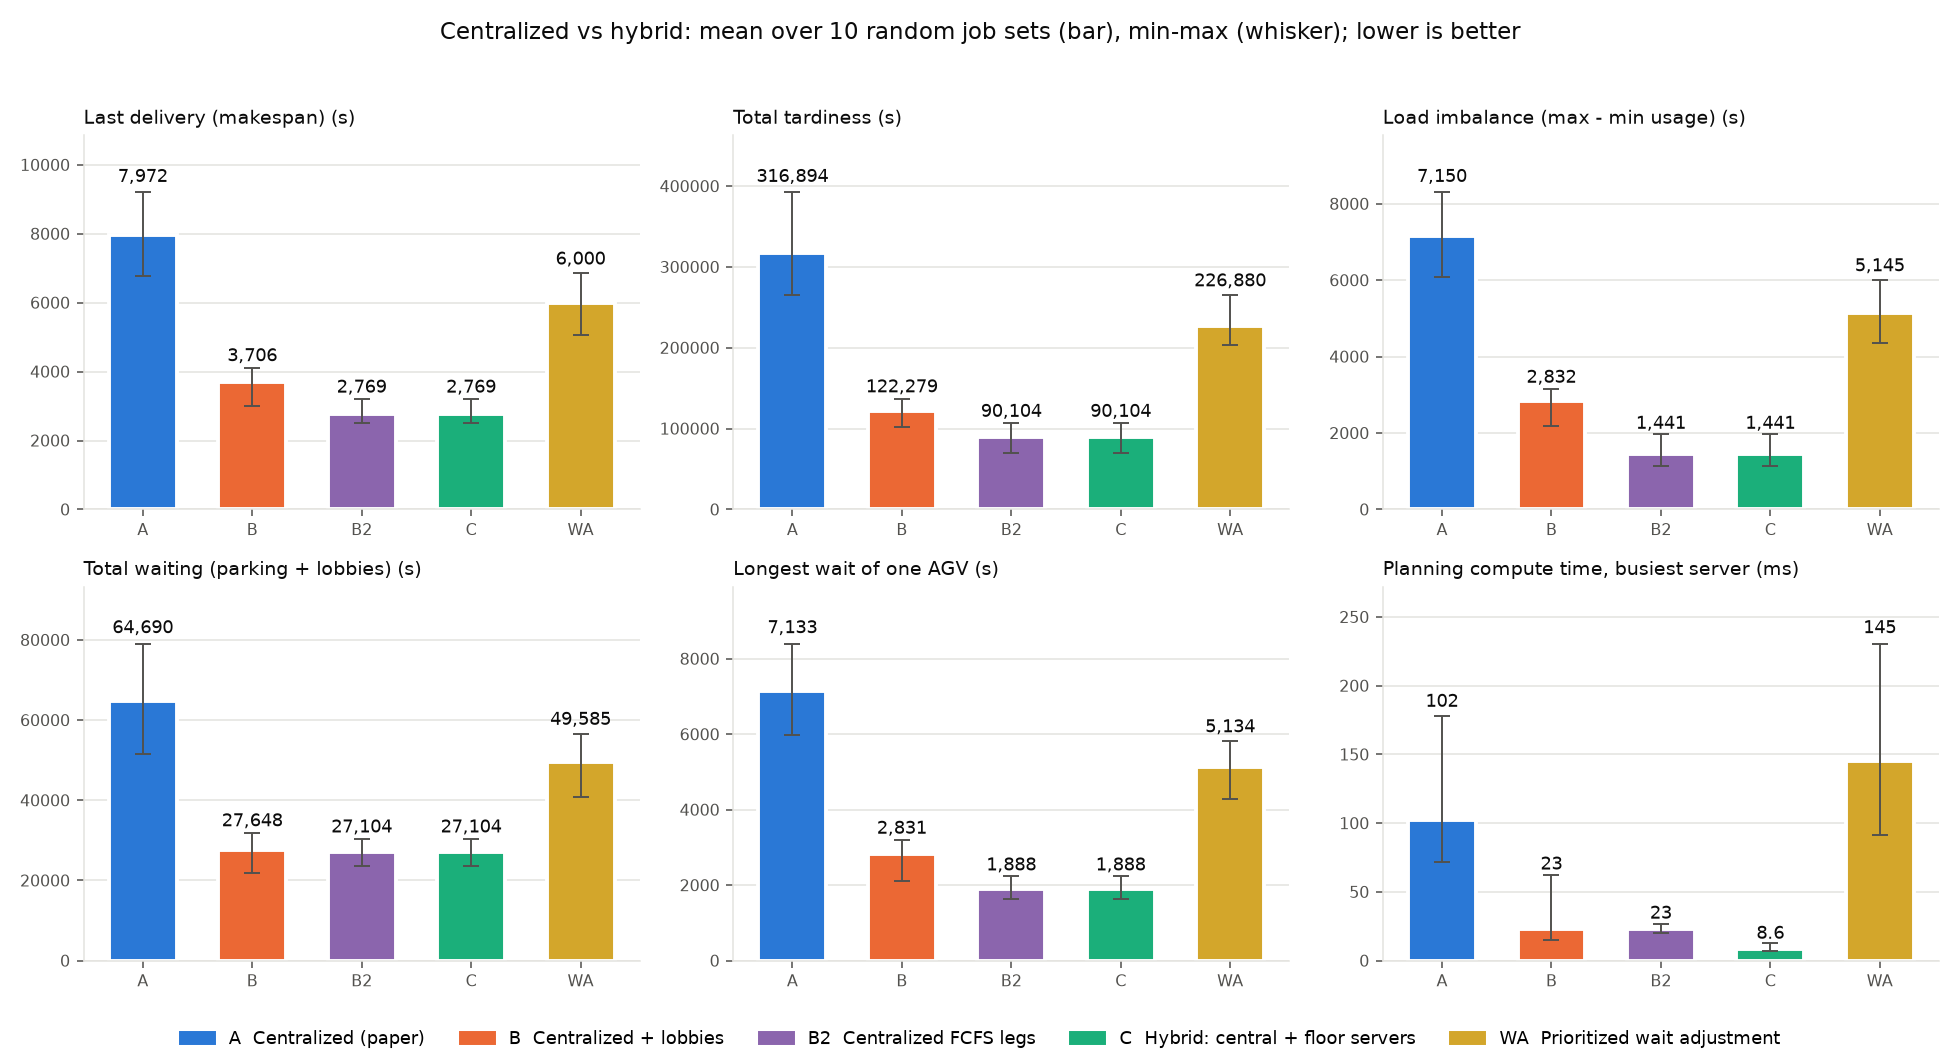
\includegraphics[width=0.98\textwidth]{../figures/fig1_compare_metrics.png}
\caption{Mean and min--max range over the ten job sets for A, B, B2, and C.}
\label{fig:main-comparison}
\end{figure*}

\begin{figure*}[t]
\centering
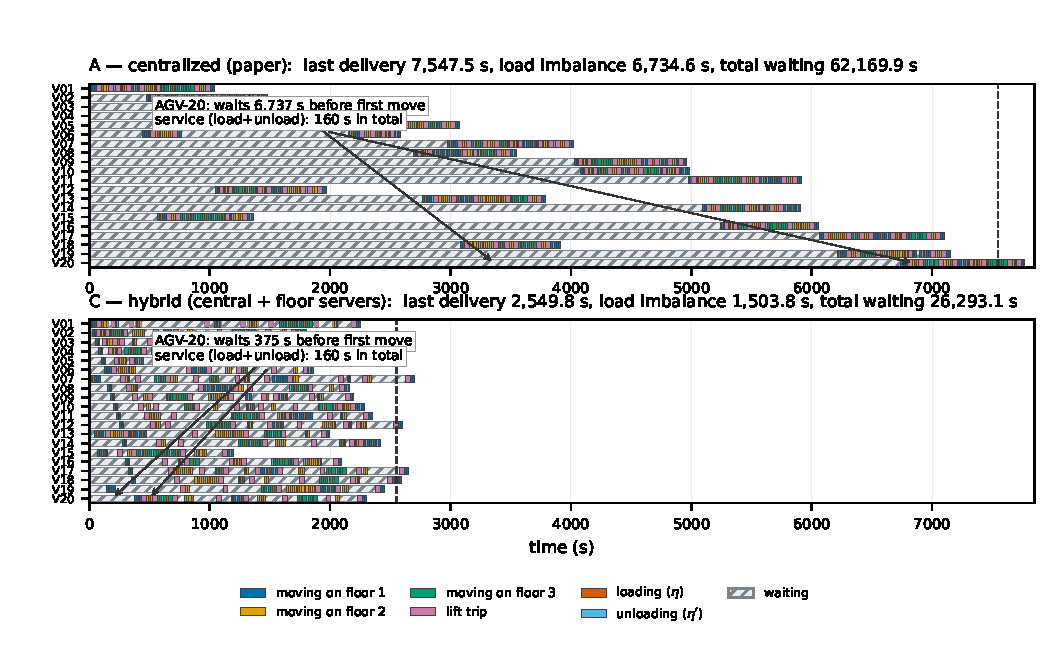
\includegraphics[width=\textwidth]{../figures/gantt_A_C_seed7.pdf}
\caption{How to read: each row is one AGV in priority order (V01 has the
highest priority), colors give the activity (moving on floor 1, 2, or 3, lift
trip, loading $\eta$, unloading $\eta'$), and hatched bars are waiting. The
panels show the seed-7 job set under A (top) and C (bottom) on a shared time
axis; dashed lines mark each panel's last delivery. What to notice: under A
the rows form a staircase of waiting that descends with priority. The
annotation marks \GanttLongWaitAgvA{}: it waits \GanttLongWaitA~s before its
first move under A but only \GanttSameAgvWaitC~s under C, while its service
time is \GanttServiceSameAgv~s in both configurations. Panel titles give the
data-derived totals: last delivery \GanttPanelALastDelivery{} versus
\GanttPanelCLastDelivery~s, load imbalance \GanttPanelAImbalance{} versus
\GanttPanelCImbalance~s, and total waiting \GanttPanelAWaitTotal{} versus
\GanttPanelCWaitTotal~s.}
\label{fig:gantt-seed7}
\end{figure*}

\begin{figure}[htbp]
\centering
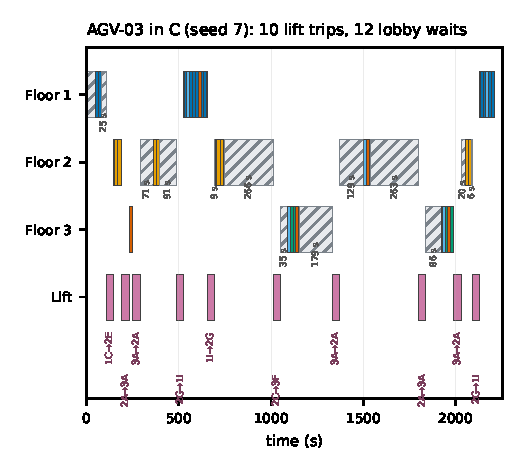
\includegraphics[width=\columnwidth]{../figures/gantt_zoom_seed7_agv-03.pdf}
\caption{How the hybrid builds one route, shown for \GanttZoomAgv{} under C on
the same seed. Rows are the three floors and the lifts; the AGV's route is cut
into floor legs joined by \GanttZoomLiftTrips{} lift trips (labelled with
their lobby-to-lobby nodes). Hatched bars at the lift-entry lobbies are lobby
waits: \GanttZoomLobbyWaits{} waits totalling \GanttZoomLobbyWaitTotal~s.
Notice the repeated pattern travel, lobby wait, lift trip: between floor legs
the AGV waits at lift lobbies rather than holding a floor node.}
\label{fig:gantt-zoom}
\end{figure}

\subsection{Fleet-size sweep}

Table~\ref{tab:fleet-sweep} gives ten-seed mean imbalance and tardiness.
Tardiness decreases with fleet size for
A at every tested step. For B it decreases through 16 AGVs, then rises from
\FleetTardBSixteen~s at 16 AGVs to \FleetTardBTwenty~s at 20. For B2 and C it
decreases slightly
from \FleetTardBtwoSixteen~s to \FleetTardBtwoTwenty~s over that final step.
Thus tardiness does not fall
monotonically in all configurations. Imbalance falls for A and rises for B,
B2, and C over this sweep. B2 and C have the same values at every tested
fleet size.

\begin{table*}[htbp]
\centering
\scriptsize
\caption{Fleet sweep: mean $\pm$ sd load imbalance and total tardiness (s), ten seeds.}
\label{tab:fleet-sweep}
% Generated by make_paper_numbers.py; do not edit.
\begin{tabular}{llrrrr}
\toprule
AGVs & Metric & A & B & B2 & C \\
\midrule
4 & imbalance (s) & $9,119\pm1,420$ & $2,043\pm377$ & $518\pm219$ & $518\pm219$ \\
4 & tardiness (s) & $602,120\pm102,189$ & $256,490\pm21,221$ & $235,718\pm14,871$ & $235,718\pm14,871$ \\
8 & imbalance (s) & $8,394\pm1,186$ & $2,346\pm334$ & $788\pm201$ & $788\pm201$ \\
8 & tardiness (s) & $453,005\pm58,101$ & $149,864\pm14,928$ & $126,223\pm12,444$ & $126,223\pm12,444$ \\
12 & imbalance (s) & $8,249\pm763$ & $2,456\pm358$ & $1,145\pm256$ & $1,145\pm256$ \\
12 & tardiness (s) & $421,464\pm50,500$ & $125,292\pm21,328$ & $100,319\pm13,957$ & $100,319\pm13,957$ \\
16 & imbalance (s) & $7,466\pm870$ & $2,715\pm316$ & $1,230\pm161$ & $1,230\pm161$ \\
16 & tardiness (s) & $348,159\pm52,200$ & $117,682\pm10,762$ & $90,343\pm9,685$ & $90,343\pm9,685$ \\
20 & imbalance (s) & $7,150\pm773$ & $2,832\pm291$ & $1,441\pm241$ & $1,441\pm241$ \\
20 & tardiness (s) & $316,894\pm41,316$ & $122,279\pm11,431$ & $90,104\pm11,447$ & $90,104\pm11,447$ \\
\bottomrule
\end{tabular}

\end{table*}

Figure~\ref{fig:fleet-sweep} shows all three fleet-sweep metrics.
\begin{figure*}[t]
\centering
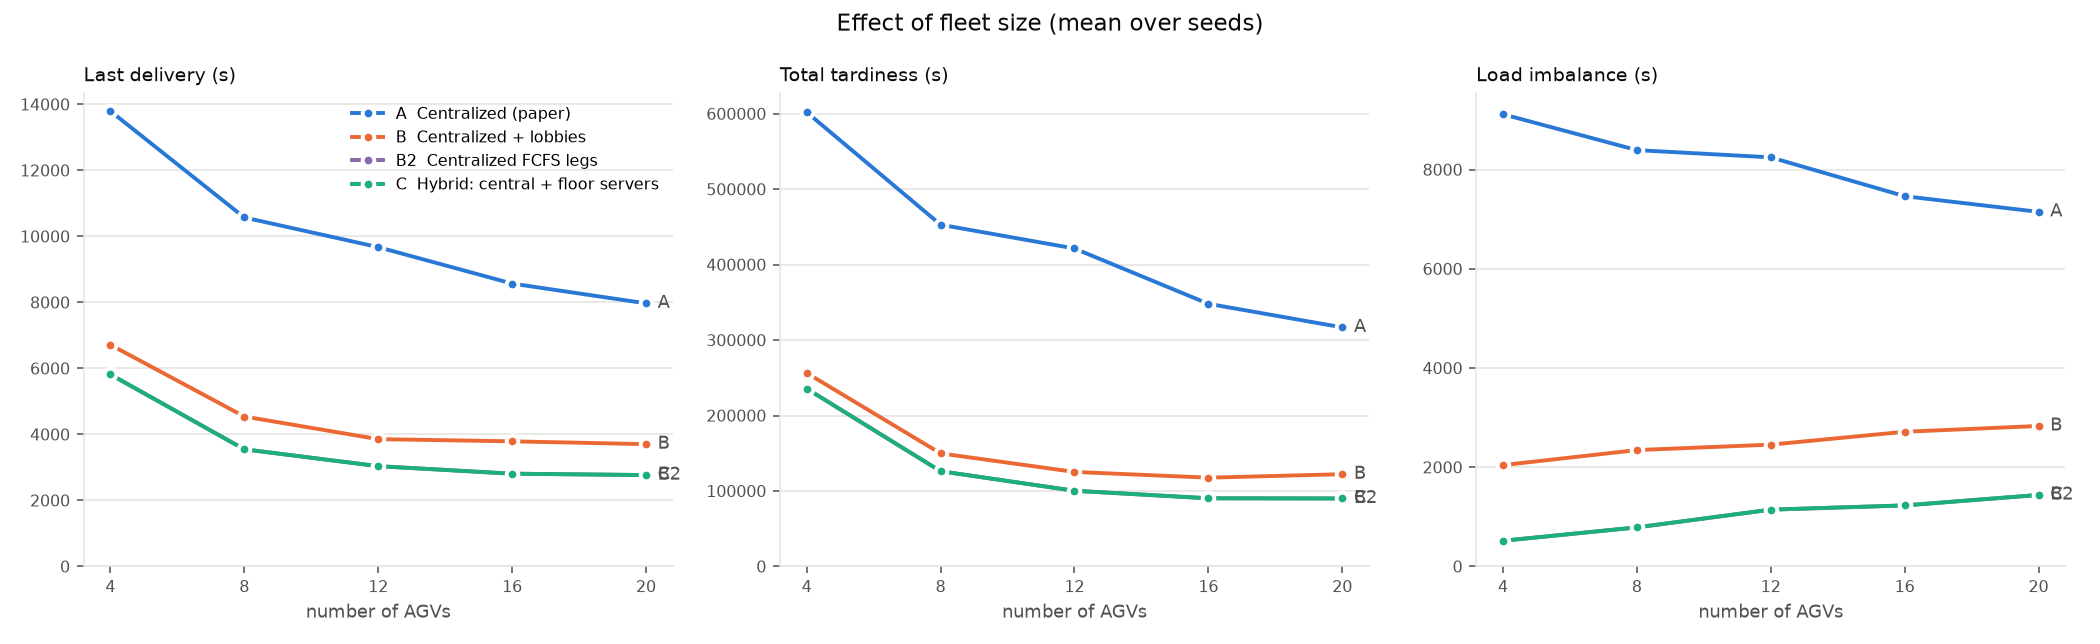
\includegraphics[width=0.98\textwidth]{../figures/fig3_fleet_size_sweep.png}
\caption{Mean makespan, tardiness, and load imbalance by fleet size over the tested seeds.}
\label{fig:fleet-sweep}
\end{figure*}

\subsection{Job-scale sweep}

The job-scale experiment fixes 20 AGVs and evaluates 50, 100, 200, and 400
jobs over seeds 1--5. Table~\ref{tab:job-scale} reports C's means and its
percentage reductions relative to A. B2 and C have identical outcomes at each
tested scale. The C-to-A reduction grows across these four tested workload
sizes for all three metrics. This is an observed trend for the tested layout,
fleet, and seeds, not a general scaling guarantee.

\begin{table*}[htbp]
\centering
\scriptsize
\caption{Job-scale means: C metrics (mean $\pm$ sd, seeds 1--5) and C reduction relative to A.}
\label{tab:job-scale}
% Generated by make_paper_numbers.py; do not edit.
\begin{tabular}{rrrrrrr}
\toprule
Jobs & C makespan (s) & C tardiness (s) & C imbalance (s) & Makespan reduction & Tardiness reduction & Imbalance reduction \\
\midrule
50 & $1,895.9\pm307.7$ & $22,311.8\pm5,964.3$ & $1,425.6\pm572.8$ & 58.0\% & 68.3\% & 66.0\% \\
100 & $2,725.3\pm137.1$ & $83,285.2\pm9,346.9$ & $1,430.3\pm141.2$ & 65.2\% & 72.9\% & 79.6\% \\
200 & $4,674.2\pm142.1$ & $360,814.5\pm6,079.8$ & $1,576.1\pm169.0$ & 72.6\% & 76.6\% & 89.8\% \\
400 & $8,541.3\pm345.2$ & $1,484,910.4\pm50,634.9$ & $2,350.0\pm437.8$ & 77.5\% & 78.9\% & 93.3\% \\
\bottomrule
\end{tabular}

\end{table*}

\subsection{Parameter sensitivity on five floors}

The sensitivity run covers a five-floor layout, 50 jobs, 10 AGVs, and three
seeds for each of 27 parameter triples: $\eta\in\{8,16,32\}$~s,
$\delta\in\{5,10,20\}$~s, and lift length in $\{20,40,80\}$~m. All
\SensitivityRows
configuration rows pass verification. Table~\ref{tab:sensitivity-c} gives
the C means at each level of one factor, averaged over the other two factors
and the three seeds.
The outcomes generally rise with larger $\delta$ and lift length in these
marginal means; the imbalance mean does not rise monotonically with $\eta$.
Because this is a finite grid of settings on one layout, it does not establish
behavior outside that grid.

\begin{table*}[htbp]
\centering
\scriptsize
\caption{Hybrid C marginal means by parameter value (mean $\pm$ sd) in the five-floor sweep.}
\label{tab:sensitivity-c}
% Generated by make_paper_numbers.py; do not edit.
\begin{tabular}{llrrr}
\toprule
Factor & Value & Makespan (s) & Tardiness (s) & Imbalance (s) \\
\midrule
$\eta$ (s) & 8 & $2,377.0\pm945.2$ & $36,979.1\pm24,312.8$ & $845.3\pm313.7$ \\
$\eta$ (s) & 16 & $2,431.2\pm882.6$ & $38,716.9\pm24,304.4$ & $892.2\pm374.0$ \\
$\eta$ (s) & 32 & $2,668.6\pm926.8$ & $42,874.4\pm24,063.4$ & $811.6\pm252.5$ \\
$\delta$ (s) & 5 & $2,290.2\pm859.0$ & $34,629.3\pm23,121.4$ & $754.9\pm290.3$ \\
$\delta$ (s) & 10 & $2,457.9\pm904.7$ & $38,250.9\pm23,793.8$ & $833.5\pm295.0$ \\
$\delta$ (s) & 20 & $2,728.8\pm960.9$ & $45,690.1\pm24,761.6$ & $960.8\pm334.3$ \\
Lift length (m) & 20 & $1,689.3\pm338.8$ & $19,697.5\pm8,465.4$ & $557.1\pm153.3$ \\
Lift length (m) & 40 & $2,307.7\pm485.5$ & $33,839.1\pm12,321.8$ & $797.2\pm169.6$ \\
Lift length (m) & 80 & $3,479.9\pm716.4$ & $65,033.7\pm20,949.7$ & $1,194.9\pm194.1$ \\
\bottomrule
\end{tabular}

\end{table*}

\subsection{Assignment baselines}

We regenerated the FCFS and random assignment baselines using the common
Algorithm 2/3 routing planner, for 100 jobs and 20 AGVs over seeds 1--3. All
five configurations passed verification on each seed. Table~\ref{tab:assign}
reports means from the per-seed baseline output.
Under this planner and these three seeds, Algorithm 1's fitness-based
assignment gives little benefit over the FCFS assignment baseline: FCFS has
slightly lower mean makespan, tardiness, and imbalance. Random assignment is
substantially worse on all three measures. This small three-seed comparison
does not establish a general ranking.

\begin{table*}[htbp]
\centering
\scriptsize
\caption{Assignment baselines: means $\pm$ sd over seeds 1--3 (100 jobs, 20 AGVs).}
\label{tab:assign}
% Generated by make_paper_numbers.py; do not edit.
\begin{tabular}{lrrr}
\toprule
Configuration & Makespan (s) & Tardiness (s) & Imbalance (s) \\
\midrule
A: Algorithm 1 assignment & $7,888.6\pm1,134.1$ & $316,407.8\pm65,925.4$ & $7,048.3\pm1,081.2$ \\
B: centralized with lobbies & $3,687.0\pm159.4$ & $120,550.8\pm14,279.8$ & $2,858.9\pm164.4$ \\
C: hybrid & $2,783.2\pm101.8$ & $84,528.3\pm12,996.4$ & $1,431.9\pm199.1$ \\
FCFS assignment & $7,750.5\pm1,267.6$ & $304,553.0\pm76,618.6$ & $6,971.3\pm1,150.7$ \\
Random assignment & $12,322.1\pm1,520.5$ & $493,263.8\pm86,185.2$ & $11,959.8\pm1,744.8$ \\
\bottomrule
\end{tabular}

\end{table*}

\subsection{Competing prioritized wait-adjustment planner}

The competing planner (WA) computes individual paths and inserts waits to
avoid conflicts using the same seeded jobs, layout, fleet, speeds, and safety
gap. In the 10-seed, 100-job, 20-AGV comparison, every WA plan passed
verification. Its mean makespan, tardiness, and imbalance were \WAMakespan~s,
\WATardiness~s, and \WAImbalance~s, respectively, compared with \MakespanC~s,
\TardinessC~s, and \ImbalanceC~s for C. The job-scale sweep also reports higher WA
means than C at 50, 100, 200, and 400 jobs. On these tested cases WA did not
outperform the hybrid; this is not evidence that it cannot do so on other
instances.

\subsection{Finite lobby capacity}

The capacity experiment evaluates B and C on three- and five-floor layouts,
100 jobs, 20 AGVs, and ten seeds. Table~\ref{tab:lobby-cap} reports B's
verified-plan counts and means when available, and C's verified counts and
means. The summary describes finite-capacity C as using conservative FCFS
tour admission, with other AGVs waiting at $\pi$ to avoid lobby wait-for
cycles. Its finite-capacity plans verify, but the resulting schedules are
much slower than the unlimited-capacity case. Some B seeds failed plan
verification; that is a planner failure in those runs, not proof that the
underlying scheduling instances are physically infeasible.

\begin{table*}[htbp]
\centering
\scriptsize
\caption{Finite-lobby results: verified runs out of ten and mean $\pm$ sd makespan / tardiness (s).}
\label{tab:lobby-cap}
% Generated by make_paper_numbers.py; do not edit.
\begin{tabular}{llrrrrrr}
\toprule
Layout & $K$ & B verif. & B makespan (s) & B tardiness (s) & C verif. & C makespan (s) & C tardiness (s) \\
\midrule
3 floor & 1 & 0/10 & n/a & n/a & 10/10 & $19,153.1\pm649.9$ & $911,565.3\pm35,190.0$ \\
3 floor & 2 & 2/10 & $4,108.9\pm188.5$ & $146,026.1\pm2,430.2$ & 10/10 & $19,153.1\pm649.9$ & $911,565.3\pm35,190.0$ \\
3 floor & 4 & 10/10 & $3,764.2\pm374.8$ & $124,813.4\pm12,984.3$ & 10/10 & $19,153.1\pm649.9$ & $911,565.3\pm35,190.0$ \\
3 floor & Unlimited & 10/10 & $3,705.9\pm309.8$ & $122,278.8\pm11,430.7$ & 10/10 & $2,768.9\pm195.8$ & $90,104.5\pm11,447.3$ \\
5 floor & 1 & 0/10 & n/a & n/a & 10/10 & $26,701.3\pm1,164.7$ & $1,294,641.3\pm72,645.6$ \\
5 floor & 2 & 0/10 & n/a & n/a & 10/10 & $26,701.3\pm1,164.7$ & $1,294,641.3\pm72,645.6$ \\
5 floor & 4 & 9/10 & $4,059.7\pm318.2$ & $134,817.4\pm19,342.2$ & 10/10 & $26,701.3\pm1,164.7$ & $1,294,641.3\pm72,645.6$ \\
5 floor & Unlimited & 10/10 & $4,014.8\pm339.4$ & $133,751.7\pm19,177.3$ & 10/10 & $3,174.2\pm299.1$ & $110,421.4\pm14,112.9$ \\
\bottomrule
\end{tabular}

\end{table*}

\subsection{Per-server state and computation}

For seed 7, the centralized planner reports \SeedSevenWindowsCentralA~windows and
\SeedSevenCpuCentralA~ms CPU on A's central server. C holds
\SeedSevenWindowsCentralC~windows and uses \SeedSevenCpuCentralC~ms on
its central server; its floor servers hold \SeedSevenWindowsFloorOneC,
\SeedSevenWindowsFloorTwoC, and \SeedSevenWindowsFloorThreeC windows and use
\SeedSevenCpuFloorOneC, \SeedSevenCpuFloorTwoC, and \SeedSevenCpuFloorThreeC~ms,
respectively. The largest C server therefore holds
\SeedSevenLargestCWindows~windows and uses \SeedSevenLargestCCpu~ms in this
seed. These seed-specific values are
distinct from the ten-seed means in Table~\ref{tab:mean-results}. The server
state and CPU comparison appears in Figure~\ref{fig:per-server}.

\begin{figure*}[t]
\centering
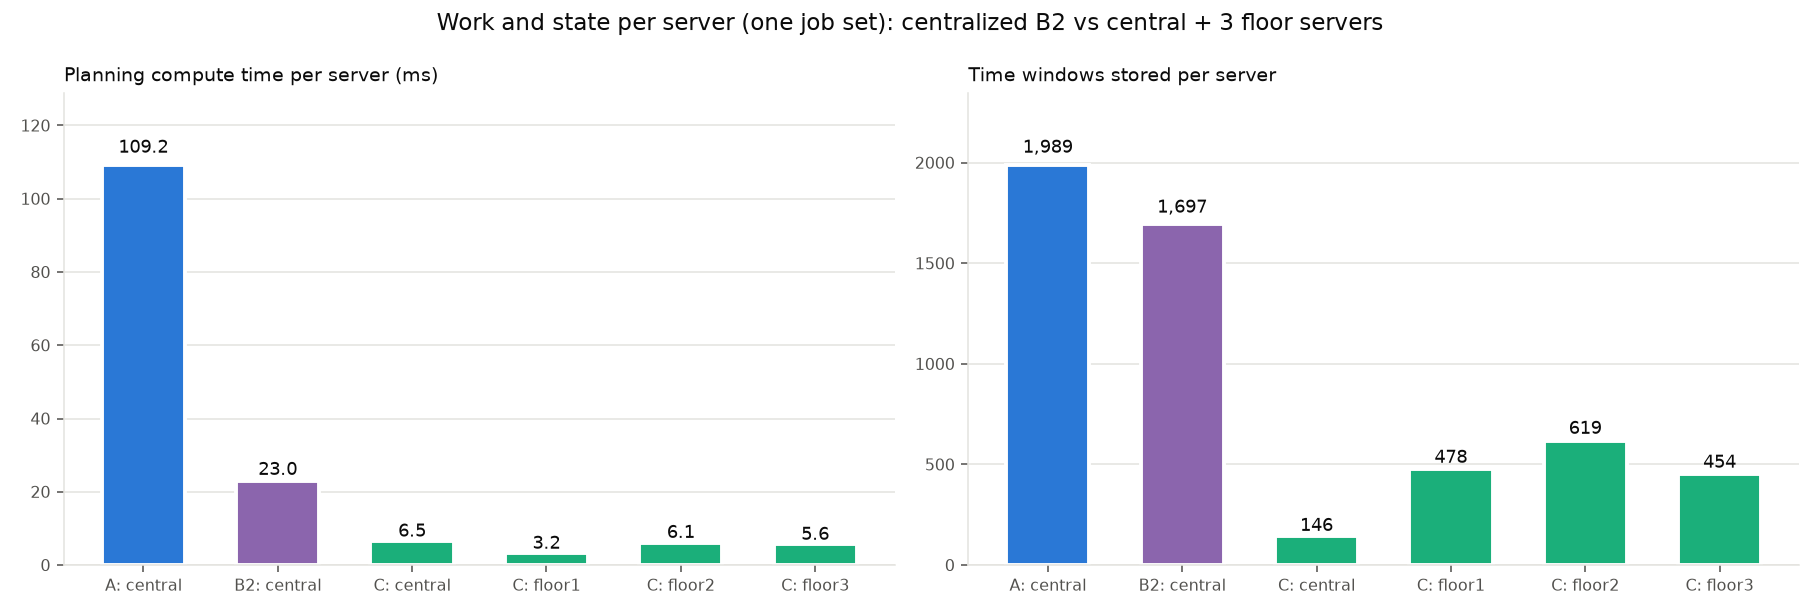
\includegraphics[width=0.98\textwidth]{../figures/fig4_per_server.png}
\caption{Per-server computation time and reservation windows for centralized B2 and hybrid C on seed 7.}
\label{fig:per-server}
\end{figure*}

\subsection{Discussion and scope}

In the tested three-floor setting, adding lobbies improves the A-to-B
comparison. Changing B to B2 changes route-leg processing to FCFS and
improves the reported scheduling outcomes. B2 and C then match schedule
metrics, so the additional floor-server split changes measured state and
computation distribution, not schedule quality, in these comparisons. The
five-floor sensitivity and lobby-capacity experiments show that outcomes
depend on parameter values and on the capacity-handling policy. Finite
capacity under the tested conservative admission rule can impose large
delays. The job-scale sweep indicates a larger C-versus-A reduction over the
four tested workloads, while the fleet sweep has the non-monotone B
tardiness result described above. None of these finite experiments establishes
performance outside the layouts, seeds, fleet sizes, and parameters tested.

